\documentclass{article}

\usepackage{arxiv}
\usepackage[utf8]{inputenc} 
\usepackage[T1]{fontenc}
\usepackage{newunicodechar}
\newunicodechar{́}{\'{}}    
\usepackage{hyperref}       
\usepackage{url}            
\usepackage{booktabs}       
\usepackage{amsfonts}       
\usepackage{nicefrac}
\usepackage{graphicx}
\usepackage{subcaption}
\usepackage{verbatim}
\usepackage{adjustbox}
\usepackage{float}
\usepackage[spanish]{babel}
\usepackage{microtype}      
\usepackage{lipsum}
\usepackage{amsmath}
\usepackage[margin=1in]{geometry}
\usepackage{multicol}
\graphicspath{ {./images/} }
\renewcommand{\refname}{Referencias}
\usepackage{caption}


\title{TP 2.1 - Generadores Pseudoaleatorios }


\author{
 Aldana Risso Patrón \\
  Universidad Tecnológica Nacional - FRRO \\
  Zeballos 1341, S2000, Argentina \\
  \texttt{rissopatronaldana7@gmail.com} \\
   \And
 Ignacio Fierro \\
  Universidad Tecnológica Nacional - FRRO \\
  Zeballos 1341, S2000, Argentina \\
  \texttt{nachofier@gmail.com} \\
  \And
 Lucía Gelmetti \\
  Universidad Tecnológica Nacional - FRRO \\
  Zeballos 1341, S2000, Argentina \\
  \texttt{luligelmetti@gmail.com} \\
  \And
 Juan Cruz Bonanno \\
  Universidad Tecnológica Nacional - FRRO \\
  Zeballos 1341, S2000, Argentina \\
  \texttt{bonanno2340@gmail.com} \\
  \And
 Franco Reggiardo Chuglar \\
  Universidad Tecnológica Nacional - FRRO\\
  Zeballos 1341, S2000, Argentina \\
  \texttt{francoreggiardo15@gmail.com} \\
  \And
 Marcos Oldani \\
  Universidad Tecnológica Nacional - FRRO \\
  Zeballos 1341, S2000, Argentina \\
  \texttt{marcosoldani1360@gmail.com} \\
}

\begin{document}
\maketitle
\begin{abstract}
El objetivo del siguiente documento es mostrar los diferentes generadores de números, diferenciando los aleatorios de los pseudoaleatorios, para estudiar los comportamientos de cada uno de ellos. Se pretende analizar cuáles son más competentes y cuáles conviene evitar.
\end{abstract}

\keywords{Simulación \and Generadores de numeros \and Análisis Estadístico \and Numeros aleatorios \and Numeros pseudoaleatorios }

\section{Introducción}
La aleatoriedad se entiende como un proceso en el cual el resultado es completamente imprevisible y depende únicamente del azar. Esta característica hace que la generación de números verdaderamente aleatorios sea una tarea compleja, ya que requiere el uso de factores externos incontrolables que aporten esa imprevisibilidad. En contraste, los números pseudoaleatorios son generados mediante algoritmos deterministas que, aunque producen secuencias sin patrones evidentes desde un punto de vista estadístico, no son verdaderamente aleatorios. Bajo las mismas condiciones iniciales, estos algoritmos generan siempre la misma secuencia de números. A pesar de esta limitación, los números pseudoaleatorios resultan extremadamente útiles en diversos campos, especialmente en estos trabajos de estudio de la simulación, donde su comportamiento estadísticamente aleatorio es suficiente para modelar fenómenos complejos.


\section{Generadores de numeros}
\subsection{Generadores de numeros aleatorios reales}

Los números completamente aleatorios (no
determinísticos) son fáciles de imaginar conceptualmente, por ejemplo podemos imaginar
lanzar una moneda, lanzar un dado, una lotería.
En general los números aleatorios se basan en alguna fuente de aleatoreidad física que
puede ser teóricamente impredecible (cuántica) o prácticamente impredecible (caótica). 
La desventaja de éstos métodos es que son costosos, tardados y no reproducibles.

\subsection{Generadores de números pseudoaleatorios}

Los números pseudoaleatorios se generan de manera
secuencial con un algoritmo determinístico. Para generarlos se utiliza la función de inicialización, que es un proceso que establece el estado inicial del generador de números pseudoaleatorios. Recibe un número (la semilla) y pone al generador en su estado inicial.
Luego hace uso de la funcion de transición, que transforma el estado del generador. Y por ultimo utiliza la función de salidas, que transforma el estado para producir un número fijo de bits (0 ó 1).
Es decir, una sucesión de bits pseudoaleatorios se obtiene definiendo la semilla y llamando repetidamente la función de transición y la función de salidas. Si se usa la misma semilla, se puede reproducir el resultado.

\subsubsection{Método de los cuadrados}

En 1946 Jon Von Neuman sugirió usar las operaciones aritméticas de una computadora para
generar secuencias de número pseudoaleatorios.
Sugirió el método de los cuadrados (middle square), para generar secuencias de dígitos pseudoaleatorios de 4
dígitos propuso:

\begin{enumerate}
    \item Se inicia con una semilla de 4 dígitos. 
    \item La semilla se eleva al cuadrado, produciendo un número de 8 dígitos (si el resultado tiene menos de 8 dígitos se añaden ceros al inicio). 
    \item Los 4 números del centro serán el siguiente número en la secuencia, y se devuelven
como resultado.
\end{enumerate}

Este generador cae rápidamente en cilcos cortos, por ejemplo, si aparece un cero se propagará por siempre.
A inicios de 1950s se exploró el método y se propusieron mejoras, por ejemplo para evitar caer en cero. Metrópolis logró obtener una secuencia de 750,000 números distintos al usar
semillas de 38 bits (usaba sistema binario), además la secuencia de Metrópolis mostraba propiedades deseables. No obstante, el método del valor medio no es considerado un método bueno por lo común de los ciclos cortos.

\subsubsection{RANDU}
RANDU fue un generador de números pseudoaleatorios ampliamente utilizado en la década de 1960, especialmente en sistemas IBM. Su implementación era simple y rápida, basada en el método congruencial lineal, con la fórmula:

\begin{equation}
    X_{n+1} = (2^{16} + 3)X_n mod(2^{31})
\end{equation}

Este algoritmo parece generar números aleatorios al principio, pero tiene fallas serias que lo hacen inadecuado para la mayoría de aplicaciones científicas o estadísticas rigurosas.

Una de las principales críticas a RANDU es su mala distribución en espacios multidimensionales. 

\subsubsection{GCL}

Los generadores como rand y RANDU se denominan generadores congruenciales. Los Generadores Congruenciales Lineales (GCL) tienen la forma:
\begin{equation}
    X_{n+1} = (aX_n + c)mod(m)
\end{equation}

Están determinados por los parámetros: 
\begin{itemize}
    \item Módulo: $m>0$ 
    \item Multiplicador: $0 \leq a < m$
    \item Incremento: $c \leq m$
    \item Semilla: $0 \leq X_0 < m$
\end{itemize}

Los generadores congruenciales lineales (GCL) fueron introducidos en 1949 por D.~H.~Lehmer y se han vuelto muy populares en la generación de números pseudoaleatorios. La calidad del generador depende en gran medida de la elección de sus parámetros.

Si se desea un periodo largo, es importante tener en cuenta que el periodo máximo del generador no puede exceder \( n \) elementos, donde \( n \) está relacionado con el módulo. Por otro lado, si se busca velocidad en la generación, un valor conveniente para el módulo \( m \) suele estar relacionado con el tamaño de palabra de la computadora, es decir, el número máximo de bits que el procesador puede manejar en un solo ciclo.

Los GCL más eficientes suelen utilizar un módulo \( m \) igual a una potencia de 2, comúnmente \( 2^{32} \) o \( 2^{64} \). De esta manera, la operación módulo se puede realizar de forma eficiente truncando todos los bits excepto los últimos 32 o 64, lo que reduce significativamente el tiempo de cómputo.


La pregunta es, ¿podemos elegir y de tal manera que logremos alcanzar el periodo máximo (\( m \))? Un
generador congruencial mixto ($c>0$) tendrá periodo completo para todas las semillas sí y sólo sí:

\begin{itemize}
    \item y son primos relativos.
    \item es divisible por todos los factores primos de m.
    \item es divisible por 4 si es divisible por 4.
\end{itemize}

Los GCLs continuan siendo utilizados en muchas aplicaciones porque con una elección cuidadosa de los parámetros pueden pasar muchas pruebas de aleatoriedad, son rápidos y requiren poca memoria.
\subsubsection{Generador de numeros pseudoaleatorios con Python}

El módulo random es una de las bibliotecas estándar de Python para la generación de números pseudoaleatorios. Proporciona funciones sencillas para generar valores numéricos dentro de intervalos específicos, así como para realizar selecciones aleatorias de elementos dentro de secuencias. Internamente, utiliza el algoritmo Mersenne Twister, conocido por su buena calidad estadística y su rapidez, aunque no es adecuado para aplicaciones criptográficas debido a su naturaleza determinista.

Por otro lado, la biblioteca NumPy, orientada al cálculo numérico de alto rendimiento, ofrece un submódulo llamado numpy.random que permite generar números pseudoaleatorios de manera más eficiente y con mayor variedad de distribuciones. A diferencia del módulo estándar random, numpy.random está optimizado para trabajar con arrays y operaciones vectorizadas, lo cual lo hace ideal para aplicaciones científicas, análisis de datos y simulaciones a gran escala.

En este trabajo hacemos uso de ambos y mostramos los diferentes resultados. Veremos cuál es más beneficioso para simulaciones, advirtiendo que NumPy está optimizado para operar con estructuras de datos más complejas y proporciona una amplia variedad de distribuciones estadísticas, mientras que random opera de manera mas simple y estandar.
      
\section{Aplicacion de generadores}
A continuación presentaremos las distintas simulaciones, con distintos metodos y generadores para analizar sus diversos resultados.

\subsection{Histogramas de Distribución}

\subsubsection{Distribución Ideal}
Se espera que las barras tengan alturas similares a lo largo de todo el rango [0,1), lo cual refleja una distribución uniforme. Una distribución de este tipo es la ideal porque implica que todos los subintervalos del rango tienen la misma probabilidad de contener un número generado. En otras palabras, no hay concentraciones ni vacíos: los valores están repartidos de forma equilibrada. Esto sugiere que el generador está funcionando correctamente, ya que no favorece ningún segmento del intervalo. Cuando además las pruebas estadísticas —como la de chi-cuadrado o la de frecuencia— dan resultados positivos, se obtiene una validación numérica que respalda lo observado visualmente en el histograma.



\newpage

\textbf{GCL con Buenos Parámetros}

Un generador bien parametrizado distribuye los valores de forma equilibrada, lo que indica buena cobertura del espacio. La uniformidad del histograma, junto con los buenos resultados en las pruebas estadísticas, demuestra que este generador es confiable para simulaciones.

\begin{figure}[H]
\centering
\includegraphics[width=0.5\textwidth]{Imagenes/distribucion_GCL (buenos parámetros).png}
\caption{Histograma con GCL con buenos parámetros.}
\end{figure}
\raggedbottom

\textbf{Cuadrados Medios}

Se espera que las barras tengan una altura similar a lo largo de todo el rango [0,1). 
Un histograma uniforme indica que el generador está produciendo números que cubren todo el espacio de manera equilibrada. Si las pruebas estadísticas (chi-cuadrado, frecuencia) son positivas, esto confirma numéricamente lo que vemos visualmente en la siguiente figura.

\begin{figure}[H]
\centering
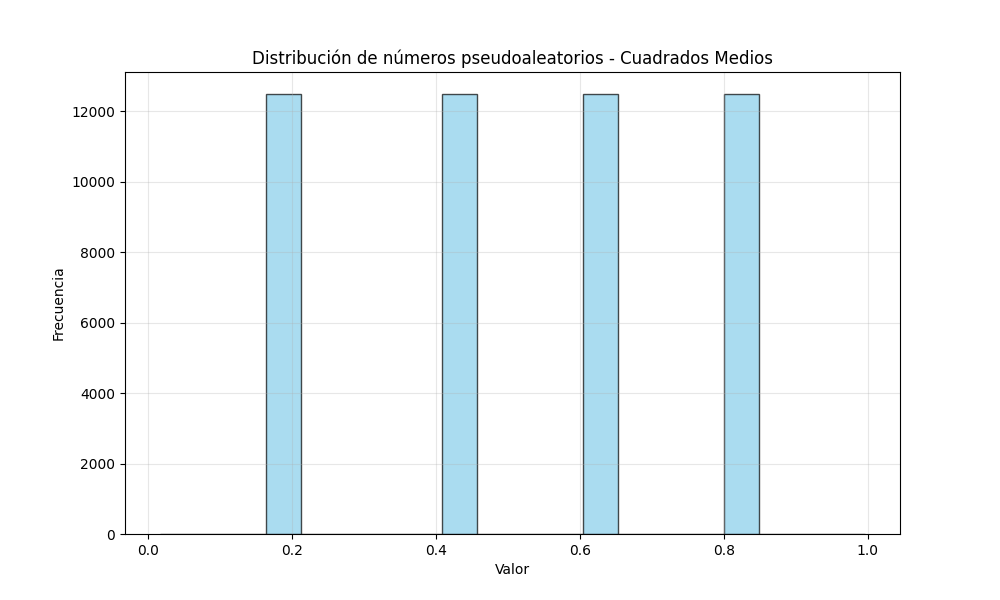
\includegraphics[width=0.5\textwidth]{Imagenes/distribucion_Cuadrados Medios.png}
\caption{Histograma con Cuadrados Medios.}
\end{figure}

\textbf{GCL tipo RANDU}

Puede mostrar cierta uniformidad en una dimensión, pero las pruebas multidimensionales fallarán
El problema de RANDU no es evidente en un histograma unidimensional, lo que demuestra que las pruebas visuales unidimensionales son insuficientes para evaluar la calidad de un generador.

\begin{figure}[H]
\centering
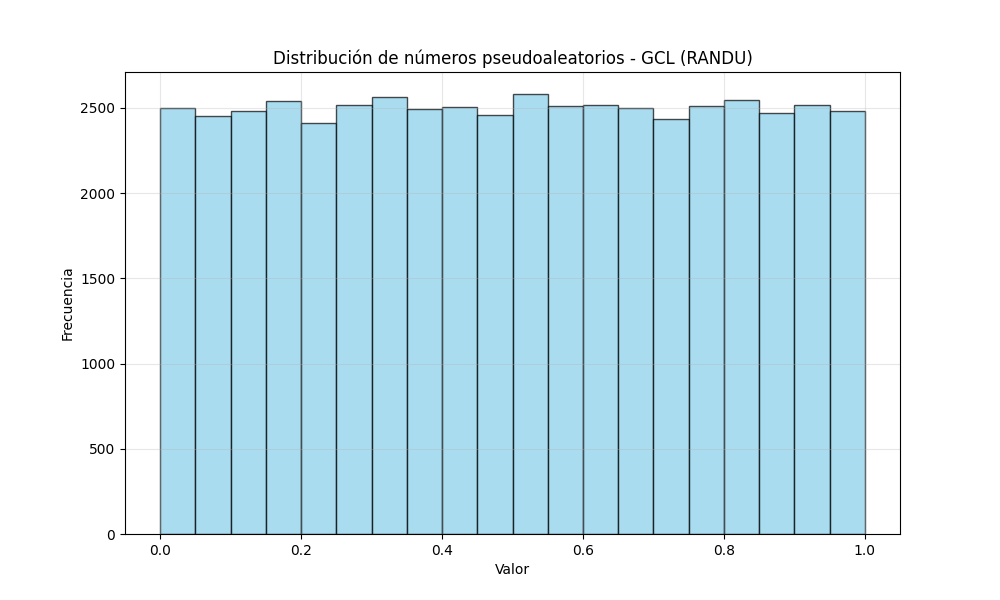
\includegraphics[width=0.5\textwidth]{Imagenes/distribucion_GCL (RANDU).png}
\caption{Histograma con GCL tipo RANDU.}
\end{figure}

\textbf{NumPy Random}

Distribución muy cercana a una uniforme ideal. Esto confirma que NumPy utiliza un algoritmo de alta calidad (basado en Mersenne Twister), que pasa todas las pruebas estadísticas y visuales necesarias para su uso en simulación científica.

\begin{figure}[H]
\centering
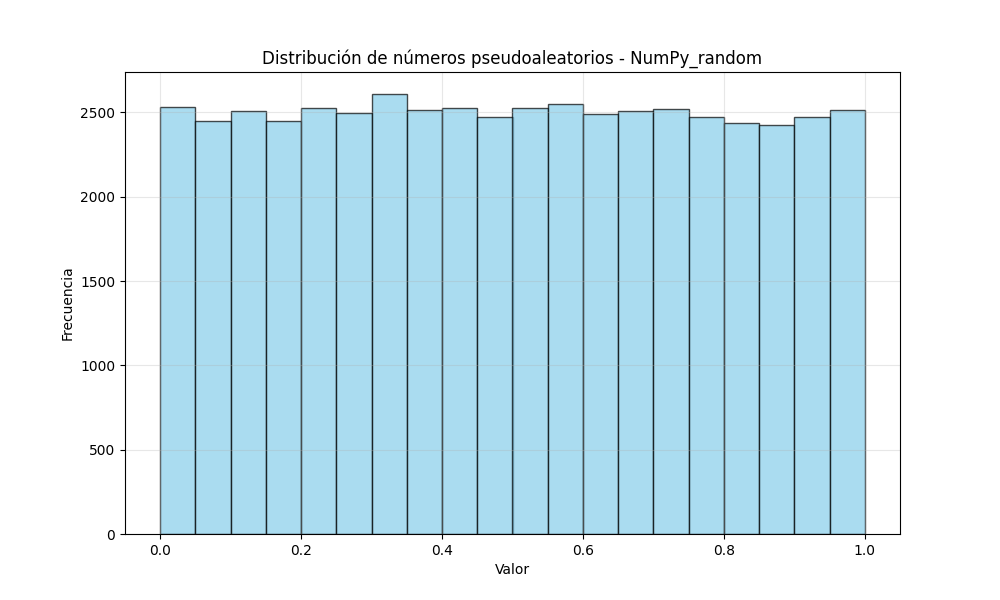
\includegraphics[width=0.5\textwidth]{Imagenes/distribucion_NumPy_random.png}
\caption{Histograma con NumPy Random.}
\end{figure}

\textbf{Python Random}

Muestra una excelente cobertura del espacio [0,1). Es un generador robusto, adecuado para tareas generales de aleatoriedad. Se basa también en el Mersenne Twister, lo que garantiza buenas propiedades estadísticas.

\begin{figure}[H]
\centering
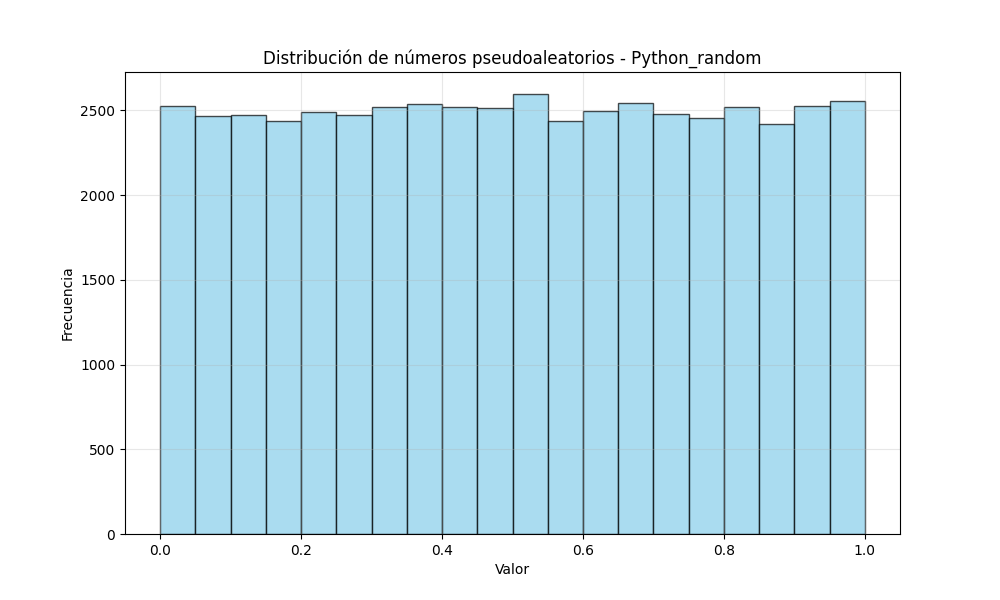
\includegraphics[width=0.5\textwidth]{Imagenes/distribucion_Python_random.png}
\caption{Histograma con Python Random.}
\end{figure}

\newpage
\textbf{Random.org}

Como se trata de números aleatorios obtenidos por fenómenos físicos reales, es lógico que su distribución sea excelente. Esta fuente es útil si se requiere aleatoriedad real, aunque su uso depende de conectividad externa.

\begin{figure}[H]
\centering
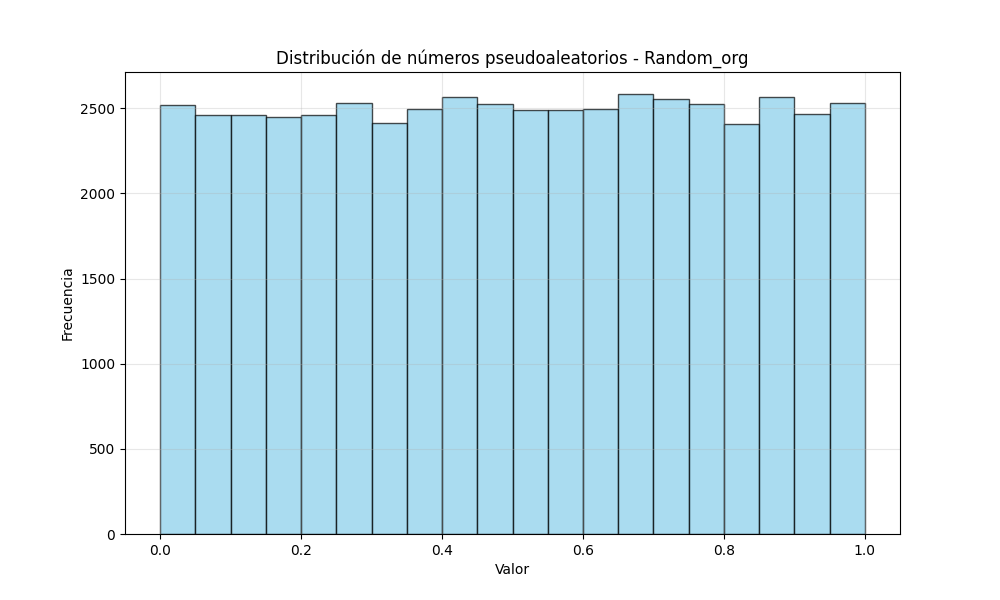
\includegraphics[width=0.5\textwidth]{Imagenes/distribucion_Random_org.png}
\caption{Histograma con Random.org.}
\end{figure}

\subsubsection{Gráficos de Series (Dispersión 2D)}
Estos gráficos muestran pares consecutivos de valores (ri, ri+1).
Como interpretación ideal observamos que, en un buen generador, los puntos deberían cubrir uniformemente el plano unitario [0,1) × [0,1) sin mostrar patrones, rayas, rejillas o agrupaciones.
Interpretación por Generador
GCL con Buenos Parámetros

En el gráfico se espera ver una nube de puntos uniforme que cubre todo el plano
No hay correlación visible entre valores consecutivos, lo que indica buena independencia estadística.

\textbf{GCL tipo RANDU}

El aspecto esperado es una distribución que puede parecer relativamente uniforme en dos dimensiones, aunque en tres dimensiones presenta problemas severos. El generador RANDU es conocido precisamente porque sus defectos no se evidencian fácilmente en pruebas bidimensionales, pero resultan catastróficos cuando se analiza en tres dimensiones.
\begin{figure}[H]
\centering
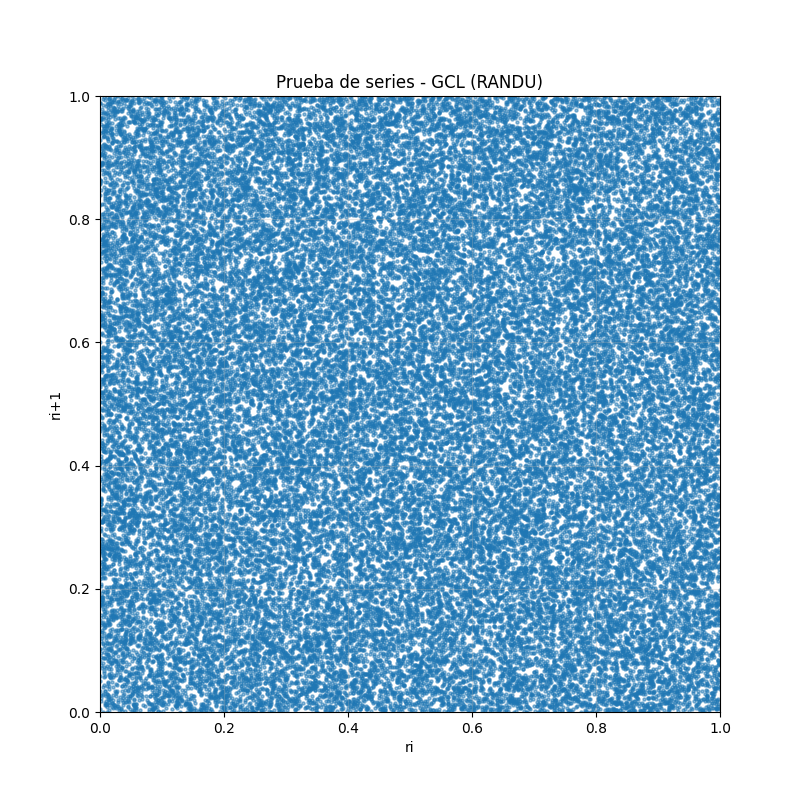
\includegraphics[width=0.5\textwidth]{Imagenes/series_GCL (RANDU).png}
\caption{Gráfico de Dispersión GCL (RANDU).}
\end{figure}

\textbf{Cuadrados Medios}

El aspecto esperado es que los puntos se agrupen cerca del origen o formen patrones muy evidentes. Esto indica una alta correlación entre valores consecutivos, lo cual es una señal clara de que el generador tiene una calidad deficiente.

\begin{figure}[H]
\centering
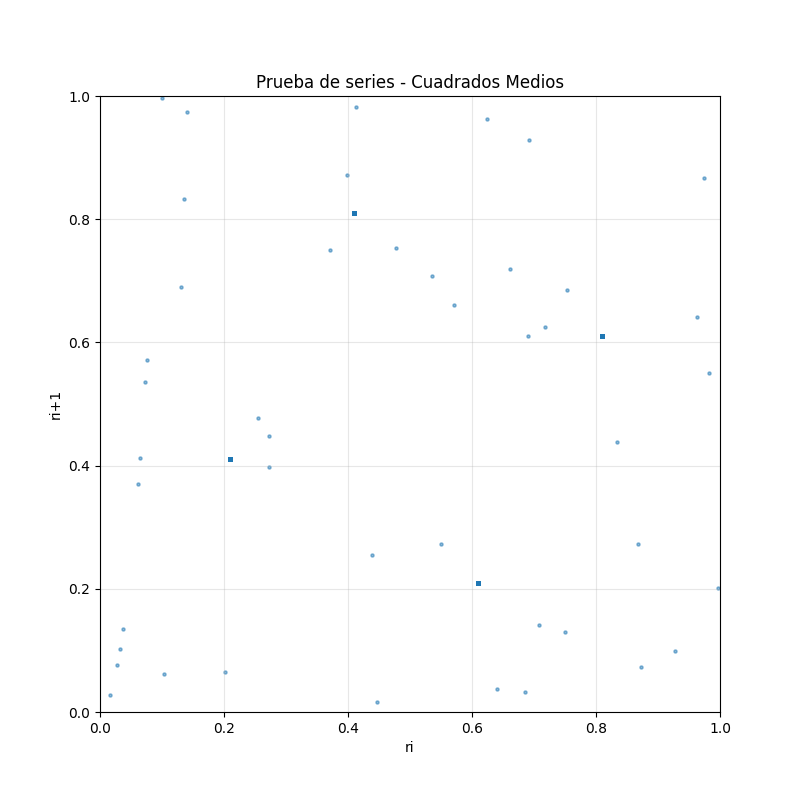
\includegraphics[width=0.5\textwidth]{Imagenes/series_Cuadrados Medios.png}
\caption{Gráfico de Dispersión Cuadrados Medios.}
\end{figure}
\textbf{Python Random | NumPy}

El aspecto esperado es una distribución uniforme sin patrones visibles.
Se aprecia una ausencia de correlación entre valores consecutivos, indicando buena calidad.
\begin{figure}[H]
\centering
\begin{subfigure}[b]{0.45\textwidth}
    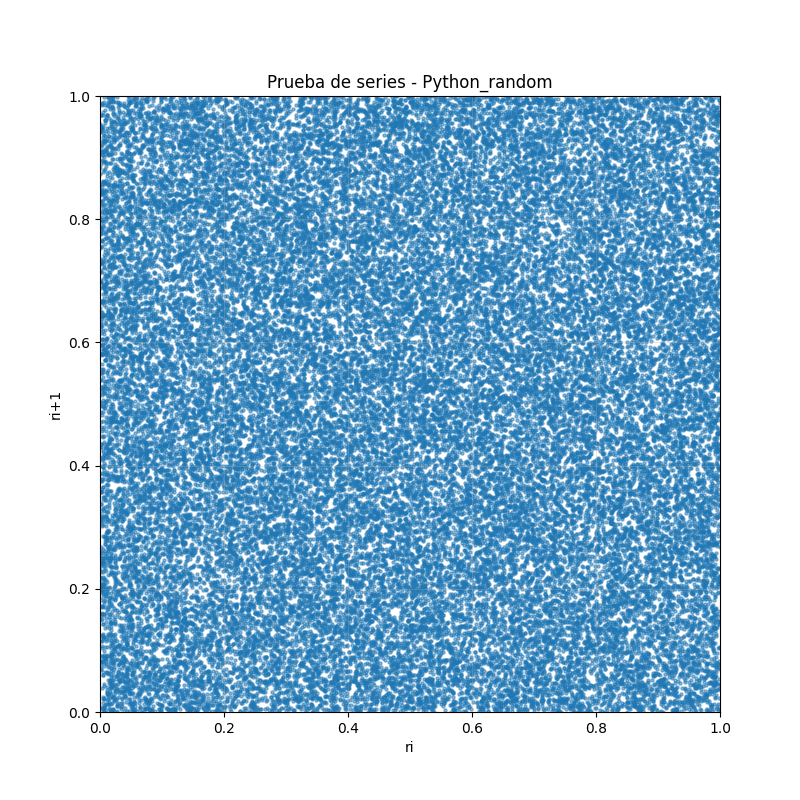
\includegraphics[width=\textwidth]{Imagenes/series_Python_random.png}
    \caption{Python Random}
\end{subfigure}
\hfill
\begin{subfigure}[b]{0.45\textwidth}
    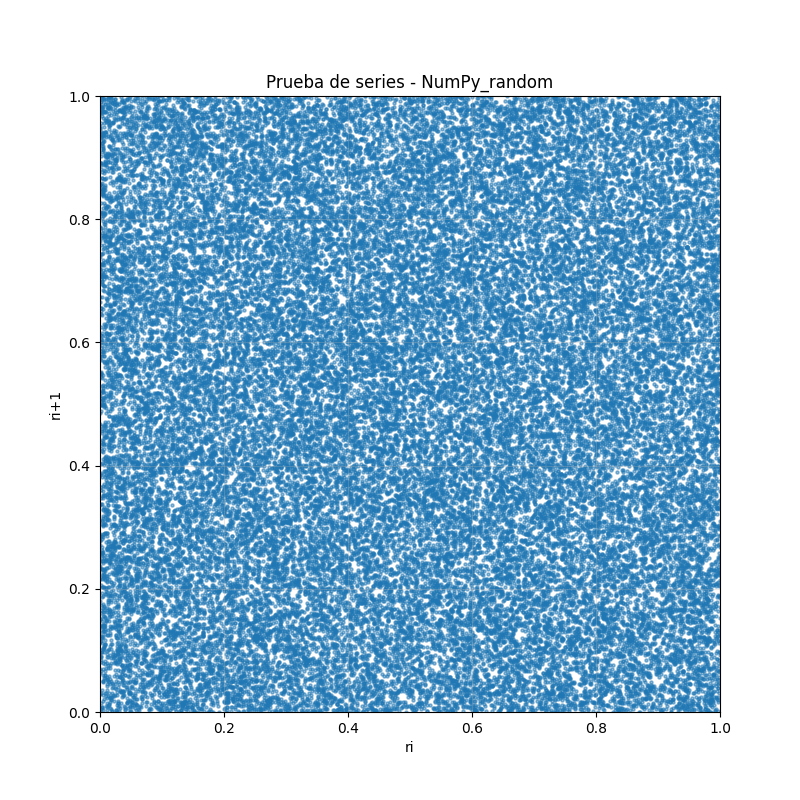
\includegraphics[width=\textwidth]{Imagenes/series_NumPy_random.png}
    \caption{NumPy Random}
\end{subfigure}
\caption{Gráfico de Dispersión de Python y NumPy.}
\end{figure}

\subsubsection{Visualizaciones 3D}
Estos gráficos muestran ternas consecutivas de valores (ri, ri+1, ri+2).
Como interpretación ideal apreciaríamos que los puntos deberían distribuirse uniformemente en el cubo unitario sin formar patrones, planos o estructuras.
A continuacion veremos las interpretaciones de cada generador.

\noindent
\begin{minipage}[t]{0.32\textwidth}
\textbf{GCL con Buenos Parámetros}  \\
El aspecto esperado es una nube de puntos tridimensional uniforme.
Se interpreta una buena independencia estadística incluso cuando se consideran tres valores consecutivos.
\end{minipage}
\hfill
\begin{minipage}[t]{0.32\textwidth}
\textbf{GCL tipo RANDU}  \\
El aspecto esperado es que la alineación de puntos en planos paralelos sea muy evidentes. Esta característica es la famosa falla del RANDU, donde los puntos se distribuyen en exactamente 15 planos dentro del espacio tridimensional, lo que revela una correlación grave y predecible entre valores sucesivos. 
\end{minipage}
\hfill
%\textbf{Cuadrados Medios}
%Aspecto esperado: Concentración de puntos en una región pequeña o formando estructuras muy regulares
%Interpretación: Alta correlación multidimensional, confirmando la mala calidad del generador.
\begin{minipage}[t]{0.32\textwidth}
\textbf{Python Random/NumPy}  \\
Se espera un aspecto de distribución uniforme en todo el cubo.
Los generadores modernos han sido diseñados específicamente para superar pruebas multidimensionales exigentes.
\end{minipage}

\begin{figure}[H]
\centering
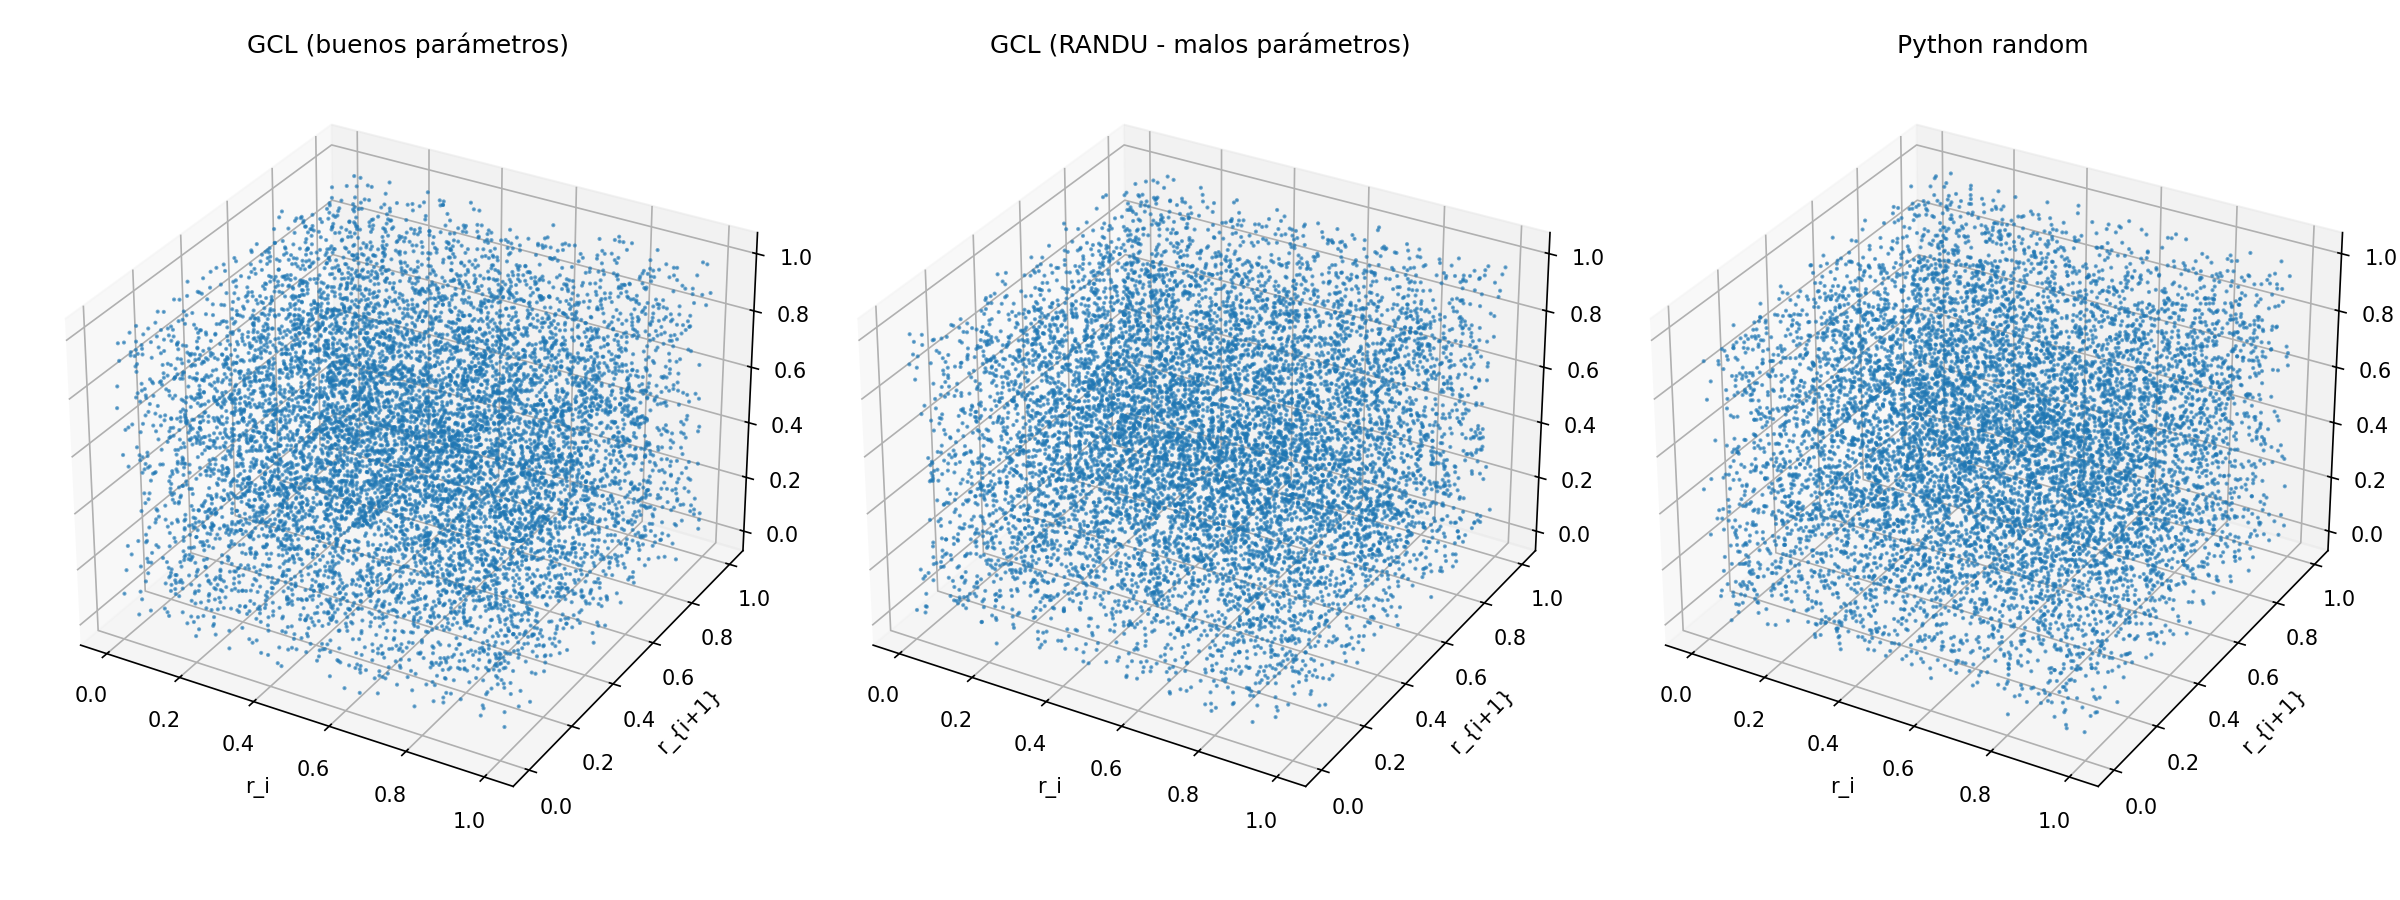
\includegraphics[width=1\textwidth]{Imagenes/comparacion_3d.png}
\caption{Gráficos de dispersión tridimensionales de GCL con buenos parámetros, GCL RANDU con malos parámetros y Python Random.}
\end{figure}

\section{Autocorrelación y Evolución Temporal}

En esta sección analizamos la autocorrelación de los números generados por cada generador, junto con la evolución temporal de los valores producidos. Estas pruebas ayudan a detectar patrones o dependencias entre valores sucesivos que no deberían estar presentes en un buen generador de números pseudoaleatorios.

\subsection{Autocorrelación}

La prueba de autocorrelación evalúa la dependencia lineal entre un valor específico en una secuencia y sus valores precedentes. En esencia, mide si un número en la secuencia está correlacionado con los números que lo anteceden en diferentes desfases o distancias.

En un generador de números aleatorios de buena calidad, el objetivo es que esta autocorrelación sea lo más cercana a cero posible para todos los desfases distintos de cero. Esto indica que cada número generado es independiente de los anteriores, una propiedad fundamental de la aleatoriedad.

La única excepción esperada es el "desfase cero", que representa la correlación de un valor consigo mismo, y que siempre será perfectamente 1.

\newpage

\begin{multicols}{2}
\setlength{\floatsep}{0pt}
\setlength{\textfloatsep}{0pt}
\setlength{\intextsep}{0pt}
\setlength{\abovecaptionskip}{0pt}
\setlength{\belowcaptionskip}{0pt}
\textbf{Cuadrados Medios:} Presenta valores de autocorrelación extremos, alternando entre 1 y -1, evidenciando una fuerte dependencia y comportamiento cíclico. Esto lo descalifica como un generador confiable.


\begin{figure}[H]
\centering
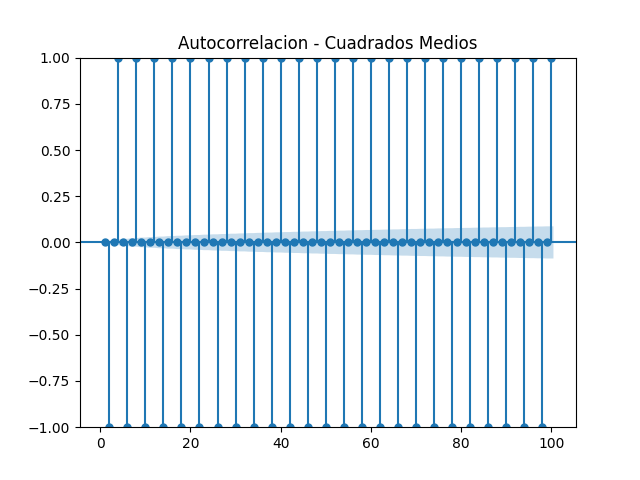
\includegraphics[width=0.4\textwidth]{Imagenes/autocorrelacion_Cuadrados Medios.png}
\caption{Autocorrelación – Cuadrados Medios}
\end{figure}


\textbf{GCL (buenos parámetros):} Muestra autocorrelaciones cercanas a cero, lo cual es deseable y refuerza su idoneidad para simulación.

\begin{figure}[H]
\centering
\includegraphics[width=0.4\textwidth]{Imagenes/autocorrelacion_GCL_(buenos parámetros).png}
\caption{Autocorrelación – GCL (buenos parámetros)}
\end{figure}



\textbf{GCL (RANDU):} Aunque las correlaciones no son tan extremas como en Cuadrados Medios, mantiene valores bajos que podrían pasar desapercibidos en esta prueba, pero se evidenciarán problemas en otras dimensiones.

\begin{figure}[H]
\centering
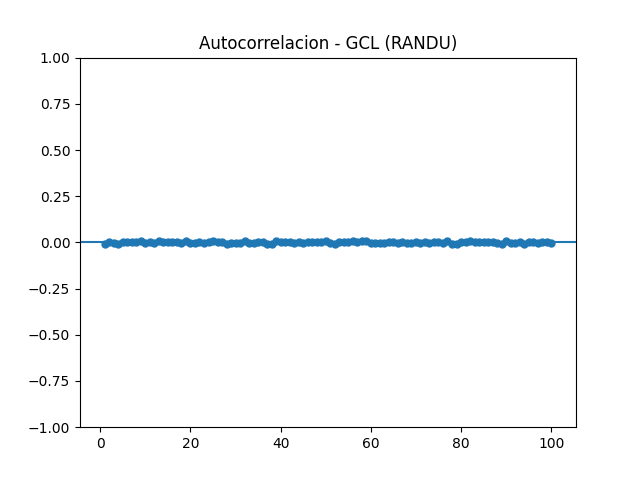
\includegraphics[width=0.4\textwidth]{Imagenes/autocorrelacion_GCL (RANDU).png}
\caption{Autocorrelación – GCL (RANDU)}
\end{figure}

\textbf{Python Random:} Se observa una buena dispersión sin patrones visibles, con autocorrelaciones cercanas a cero.

\begin{figure}[H]
\centering
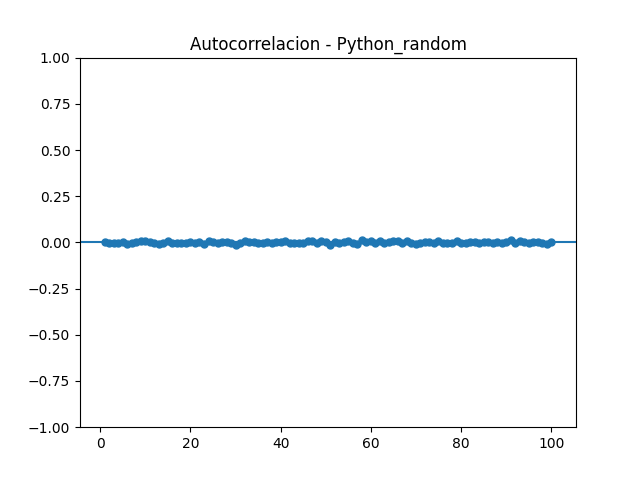
\includegraphics[width=0.4\textwidth]{Imagenes/autocorrelacion_Python_random.png}
\caption{Autocorrelación – Python Random}
\end{figure}

\textbf{NumPy Random:} Muestra comportamiento similar al anterior, con autocorrelaciones cercanas a cero y sin estructura.

\begin{figure}[H]
\centering
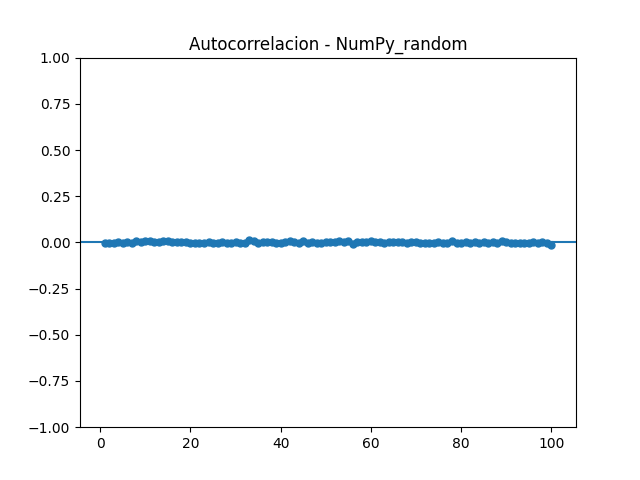
\includegraphics[width=0.4\textwidth]{Imagenes/autocorrelacion_NumPy_random.png}
\caption{Autocorrelación – NumPy Random}
\end{figure}

\textbf{Random.org:} Al provenir de un generador aleatorio verdadero, sus autocorrelaciones son mínimas y distribuidas sin tendencia.

\begin{figure}[H]
\centering
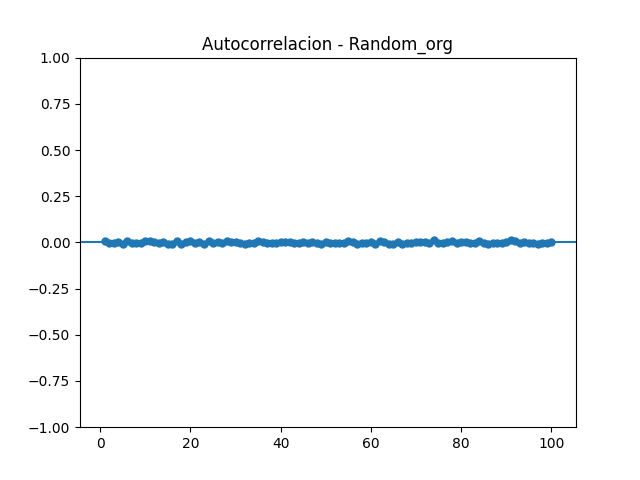
\includegraphics[width=0.4\textwidth]{Imagenes/autocorrelacion_Random_org.png}
\caption{Autocorrelación – Random.org}
\end{figure}
\end{multicols}

\subsection{Evolución Temporal de Cuadrados Medios}

Este gráfico muestra cómo los valores generados por el método de los Cuadrados Medios tienden a estabilizarse rápidamente en pocos valores, lo que evidencia su escasa capacidad para producir variabilidad. Esto coincide con la observación previa de que este método tiende a colapsar en ciclos muy cortos o valores fijos, comprometiendo gravemente la aleatoriedad de la secuencia.

\begin{figure}[H]
\centering
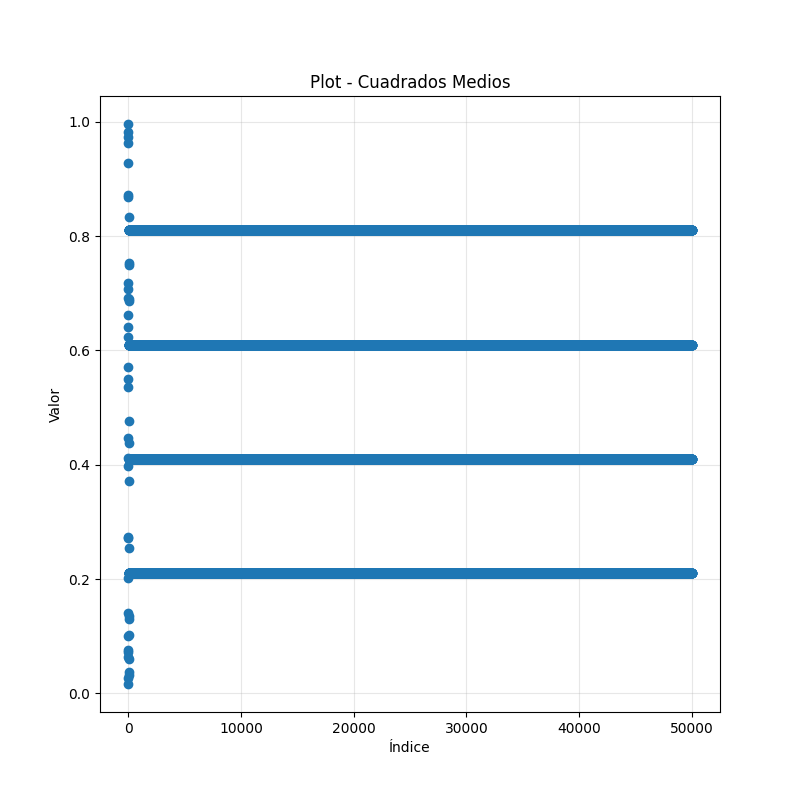
\includegraphics[width=0.5\textwidth]{Imagenes/plot_Cuadrados Medios.png}
\caption{Evolución del valor en función del índice para Cuadrados Medios}
\end{figure}

\section{Conclusión}
El análisis realizado evidencia que no todos los generadores de números pseudoaleatorios son adecuados para simulaciones. Métodos históricos como Cuadrados Medios y el GCL con parámetros tipo RANDU presentan comportamientos claramente deficientes, los cuales se reflejan tanto en pruebas estadísticas como en gráficos de distribución, series y autocorrelación. Estos generadores no logran reproducir la variabilidad esperada, mostrando patrones, ciclos cortos o concentraciones de valores que comprometen su utilidad en contextos de simulación.

Por el contrario, los generadores modernos como Python random, NumPy.random y Random.org mostraron un desempeño robusto, generando secuencias bien distribuidas, sin correlaciones visibles y con una calidad estadística adecuada. Este contraste deja en evidencia por qué los métodos modernos superan ampliamente a los enfoques clásicos.

Además, el caso particular del generador RANDU demuestra la importancia de aplicar pruebas en múltiples dimensiones, ya que algunas deficiencias sólo se manifiestan en contextos tridimensionales. También se destaca la correlación entre los análisis gráficos y las pruebas estadísticas, que deben emplearse de forma complementaria. Por último, incluso dentro de una misma familia de algoritmos, como los GCL, la correcta elección de parámetros es fundamental para garantizar la calidad del generador.

\newpage
\bibliographystyle{unsrt}  
\begin{thebibliography}{99}

\bibitem{simulaciongithub}
Aldana Risso Patrón. \textit{TP 2.1 - Generadores Pseudoaleatorios}.\\
Disponible en: \url{https://github.com/AldanaRP/TPSimulacion}


\bibitem{bacchini2018}  
Bacchini, H. \textit{Introducción a la Probabilidad y a la Estadística}.\\
Universidad de Buenos Aires, Facultad de Ciencias Económicas, 2018.\\
Disponible en: \url{http://bibliotecadigital.econ.uba.ar/download/libros/Bacchini_Introduccion-a-la-probabilidad-y-a-la-estadistica-2018.pdf}

\bibitem{numpyfromw3schools}
W3Schools \textit{NumPy Random Module for Python}.\\
Disponible en: \url{https://www.w3schools.com/python/numpy/numpy_random.asp}

\bibitem{statisticaltestpaper}
 Nist Paper\textit{A Statistical Test Suite for Random and Pseudorandom Number Generators for Cryptographic Applications(Paper)}.\\
Disponible en: \url{https://www.nist.gov/publications/statistical-test-suite-random-and-pseudorandom-number-generators-cryptographic}

\end{thebibliography}

\end{document}
